\documentclass[10pt,a4paper]{report}

\usepackage[top=2cm, bottom=2cm, left=2.5cm, right=2cm]{geometry}
% graphics images
\usepackage[pdftex]{graphicx}
\usepackage[toc,page]{appendix}
\usepackage{slashbox}
% 1.5 line spacing
\usepackage{setspace}
\usepackage{tabu}
\usepackage{tabularx}
\onehalfspacing
% maths symbols
\usepackage{amsmath, amsthm, amssymb,amsfonts}
% plot math functions
\usepackage{pgfplots}
\pgfplotsset{width=8cm,compat=1.9} % suggested setting
% table package
\usepackage{multirow}
% cross reference
\usepackage{hyperref}
% citation style
\usepackage[square,sort,comma,numbers]{natbib}
\usepackage{tikz,colortbl}
\usetikzlibrary{calc}
\usepackage{zref-savepos}
\usepackage[bf,small,tableposition=top]{caption}
\usepackage{subfig}
\usepackage{float}
\usepackage{url}
\usepackage{subfig}
\usepackage{listings}
\usepackage{wrapfig}
\usepackage{multicol}
\usepackage[section]{placeins}

%%%%%% OPTIONAL
% latex table generator : http://tablesgenerator.com/
%%%%%%%

\definecolor{codegreen}{rgb}{0,0.6,0}
\definecolor{codegray}{rgb}{0.5,0.5,0.5}
\definecolor{codepurple}{rgb}{0.58,0,0.82}
\definecolor{backcolour}{rgb}{0.95,0.95,0.92}

\lstdefinestyle{mystyle}{
    backgroundcolor=\color{backcolour},   
    commentstyle=\color{codegreen},
    keywordstyle=\color{magenta},
    numberstyle=\tiny\color{codegray},
    stringstyle=\color{codepurple},
    basicstyle=\footnotesize,
    breakatwhitespace=false,         
    breaklines=true,                 
    captionpos=b,                    
    keepspaces=true,                 
    numbers=left,                    
    numbersep=5pt,                  
    showspaces=false,                
    showstringspaces=false,
    showtabs=false,                  
}

\setlength\parindent{4em} % yes indent
\setlength{\parskip}{1em}

\lstset{style=mystyle}
\begin{document}

\begin{titlepage}
\begin{center}

% school logo

\includegraphics[width=0.3\textwidth]{image/ntu_logo.png} \hfill 
\includegraphics[width=0.3\textwidth]{image/uoe_logo.png}
\\[2cm]

\includegraphics[width=0.6\textwidth]{image/lkc_logo.png}
\\[4cm]

% project title
\uppercase{\textbf{\Large{
Debugging Lung Diseases: Applying mathematical techniques, involving modelling, data integration and machine learning for precision medicine \\[2cm]
Qualifying Examination Report}}}
\\[2cm]

% submited by ...
\uppercase{
\textbf{
Submitted by: Jayanth Kumar Narayana
}
\\
\textbf{
Matriculation Number : G1902804D
}
\\
\textbf{
	Supervisor : Asst. Prof. Sanjay Chotirmall
}
\\
\textbf{
	Co-Supervisor: Prof. Krasimira Tsaneva-Atanasova
}}

\vfill

% Bottom of the page
\textsc{\bfseries Lee Kong Chian School of Medicine, Singapore}


\end{center}
\end{titlepage}
\tableofcontents
\newpage
\listoffigures
\newpage
\listoftables
\newpage
% cover
\setcounter{page}{1}
\pagenumbering{arabic}

\chapter*{Introduction}
\addcontentsline{toc}{chapter}{Introduction}

Understanding how individual people respond to medical therapy is a crucial facet of improving the odds ratio that interventions will have a positive impact. Reducing the non-responder rate for intervention or reducing complications associated with a particular treatment is the next stage of for any medical advance. The Precision Medicine Initiative, launched in January 2015, set the stage for enhanced collaboration between researchers and medical professionals to develop next-generation techniques to aid patient treatment and recovery and increased the opportunity for impactful pre-emptive care. The microbiome plays a crucial role in health and disease, as it influences endocrinology, physiology, and even neurology, altering the outcome of many disease states, including its ability to augments drug response and tolerance.

Therefore, in precision medicine, the focus is on the identification of effective approaches for particular patients based on their genetic, lifestyle and environmental factors. Asian and European phenotypes of respiratory disease and infection are unique and therefore require such precision. While such approaches have been successfully employed to investigate contrasting clinical phenotypes; and by disease trajectories, little is known about `precision through microbes'. Precision medicine can be applied to the lung microbiome that includes both bacteria and fungi and their associated metabolic states. These `microbial fingerprints' permit patient stratification and we can identify particular disease phenotypes associated with clinical outcomes potentially amenable to precision and individualised intervention. It is clear that our microbes tell us something about disease, something representing a potential target for clinical intervention. During my PhD, I aim to extend and explore this in the context of pulmonary microbiome and lung-diseases. 

I aim to accomplish this by fulfilling the below objectives: 
\begin{enumerate}
	\item Model mathematically microbiome and mycobiome populations and their interactions across a range of pulmonary disease states: I plan to achieve this by developing computational approaches to identify mathematically significant co-operative and competitive relationships within and between species. There is also a scope for spatio-temporal modelling of the microbiome and mycobiome across various sites in the body, and study its effect on lung diseases.
	\item Develop mathematical models and tools using machine learning techniques to clinical settings in diagnosis, prognosis and predicting disease progression of patients using the pulmonary microbiome in respiratory disease states.
	\item Finally, using microbial metabolic datasets, I will further extend the developed models to take into account the affected pathways and signalling networks. This will also power our microbial airway interaction models and provide therapeutic and pharmaceutical relevance to their in vivo relationships. 
\end{enumerate}

At this point, during the submission of my Qualifying Examination report, I have accomplished the first part of my objective addressing and developing tools that capture interactions between microbes. This work is further reported in this document as two chapters with the first chapter focusing on the developed method ``Integrative microbiomics'': codified as an online webtool (\url{https://integrative-microbiomics.ntu.edu.sg/})  which when applied to pulmonary microbiome in bronchiectasis reveals a disrupted interactome. This chapter is written as a manuscript and has been submitted to Nature Medicine for publication as an original article. The second chapter of this report focuses on the application of the developed method to evaluate the `lung-gut' axis in bronchiectasis. We report the first study of the `lung-gut' axis in bronchiectasis and show a microbial dysregulation of the ‘lung-gut’ axis in high-risk bronchiectasis. 
\newpage
\chapter{``Integrative microbiomics" reveals a disrupted interactome in bronchiectasis exacerbations}
\section{Introduction}

The term microbiome is used to refer to the collection of genes within a community of microbes (including bacteria, fungi, virus, protists and bacteriophages). In the last few years, microbiome research has helped us gained new insights into how microbes shape our human biology and have brought paradigm-shifting implications for translational research and clinical care. The human microbiota is crucial for our body to maintain its homeostasis. Disruption of this can lead to diseases such as obesity, inflammatory bowel disease, malnutrition, Parkinson's, Autism, Asthma, dental caries, bacterial vaginosis, and depression \cite{Knight2017}.  Currently, microbiome researchers use culture-independent techniques that involve DNA sequencing to derive the microbiome. Broadly, the community taxonomy/microbiome can be identified using two approaches (see Figure\ref{fig1}) 1) Targeted and 2) Metagenomic. Targeted sequencing approach uses the PCR amplified, target gene markers (16S rRNA in case of bacteria or ITS in case of Fungi) derived from the samples to reference it against gene-marker databases (Silva, Green Genes, etc.). In contrast, the metagenomic sequencing approach directly sequences the whole community DNA and compares it to reference genomes \cite{Morgan2012}.

\begin{figure}[ht]
	\centering
	\includegraphics[width=0.5\textwidth]{./image/introduction.png}
	\caption{A figure illustrating the different sequencing approaches used to derive the human microbiome, consisting of interacting bacteria, fungi and viruses. Adapted from: \cite{Morgan2012}}
	\label{fig1}
\end{figure}

Present microbiome studies focus on a single profile of the human microbiome in isolation, even though bacteria, fungi and viruses coexist and interact in the body as a community. Thus, it is essential to look at these biological components together in an integrated fashion to understand more holistically the true underlying in vivo state. However, one of the primary reasons for the lack of multi-biomic research is the lack of methods to merge microbiome datasets and integrative analysis. Consequently, I tried addressing some of these challenges in my master's thesis, using microbiome datasets derived from bronchiectasis patients as an example. Bronchiectasis is a chronic inflammatory respiratory disease associated with progressive, irreversible dilatation of the airway. It is crucial to study bronchiectasis because in most cases it is known to be idiopathic(unknown cause) \cite{pmid29478908} and it is a significant contributor to lung diseases globally with a substantial four-fold higher predominance in Asian populations \cite{Seitz2012}. Exacerbation in bronchiectasis is defined as the acute episode of progressive worsening of symptoms including shortness of breath and cough. 
\begin{figure*}[!h]
	\centering
	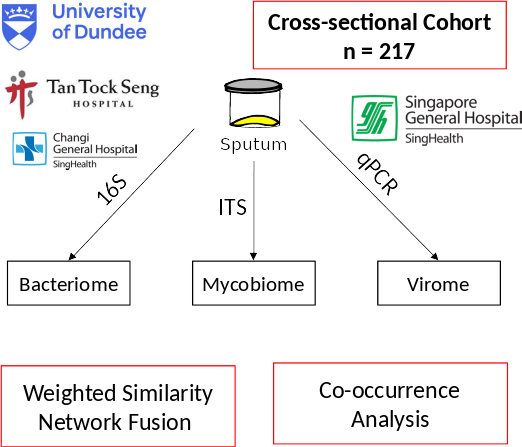
\includegraphics[width=0.50\textwidth]{./image/methods_masters.png}%
	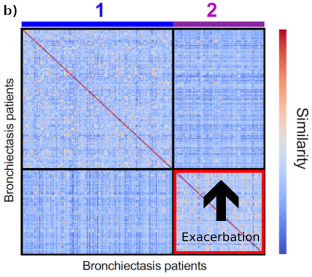
\includegraphics[width=0.50\textwidth]{./image/Res2.png}\\
	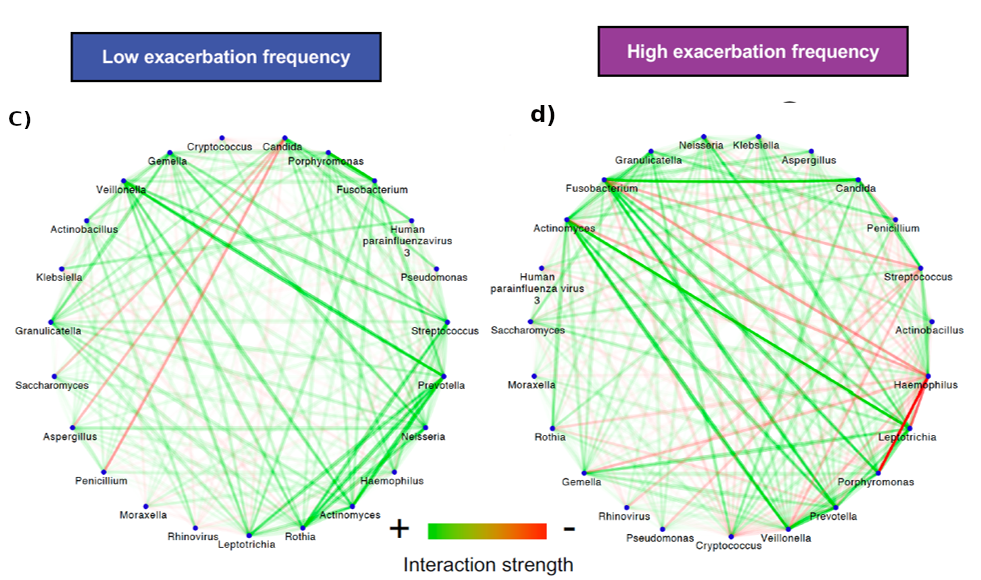
\includegraphics[width=\textwidth]{./image/Res3.png}
	\caption{(a) A schematic representing, overview of analysis performed on the CAMEB cohort (n=217). Methodologies: Weighted SNF and Co-occurrence analysis were used for microbiome integration and intreactome construction. (b) A patient similarity matrix with each cell representing the integrated similarity between patients. Two clusters of low (black) and high (red) risk patients identified by wSNF are highlighted by boxes. Visualization of the interactome of low (c) and high (d) risk clusters. Interactions between microbes are	classified as negative if the sign of the edge weights between them is negative (coloured red) with positive interactions indicated by green colouration. The strength of the interaction is indicated by the colour depth}
	\label{fig2}
\end{figure*}

Previously in my master's thesis, I developed weighted similarity network fusion (wSNF) to allow weightage of input datasets during integration, otherwise unaccounted by conventional SNF \cite{Wang2014}. Ensemble-based co-occurrence analysis strategy developed by Faust et al. \cite{Faust2012} was extended to allow weightage of individual methods in the ensemble along with other modification to better infer microbial association networks. Microbiome and Mycobiome derived using targeted amplicon sequencing of the 16S and ITS regions from the sputum samples of the CAMEB cohort \cite{Mac1800766}; virome from qPCR on an extensive panel of 17 respiratory viruses, were used as the example dataset to integrate the microbiomes (Figure\ref{fig2}a). Multi-biome (Microbiome, Mycobiome and Virome) integration by wSNF identifies a high-risk exacerbation cluster with increased precision (Figure\ref{fig2}b). Co-occurrence network analysis of this high-risk cluster revealed an elevated antagonistic interactome with reduced alpha-diversity (Figure\ref{fig2}c) \cite{Narayana2019}.

Having developed the wSNF and shown its increased precision to identify exacerbators (clinical outcomes); here in this chapter of my PhD thesis, I attempt to extend my results further. I aim to develop a web tool to enable users to integrate their microbiome datasets and to illustrate its advantages using publicly available microbiome datasets. The tool would motivate clinicians and microbiome researchers to explore multi-biome strategies for their research questions and aid them in integrating their datasets. Secondly, I aim to study exacerbation events, antimicrobial perturbations and ``Time to next exacerbation" using the developed ``Interactome" framework. Thirdly, I aim to validate the ``high-risk" exacerbation cluster of Bronchiectasis patients and its ``interactome" as derived in my previous work \cite{Narayana2019} using an alternate sequencing approach: metagenomics. Further, we also identify an interaction from the interactome of the high and low-risk clusters and validate it experimentally. 
\section{Methods}

\subsection{Integrative-microbiomics, a webtool}
\begin{figure*}[h]
	\centering
	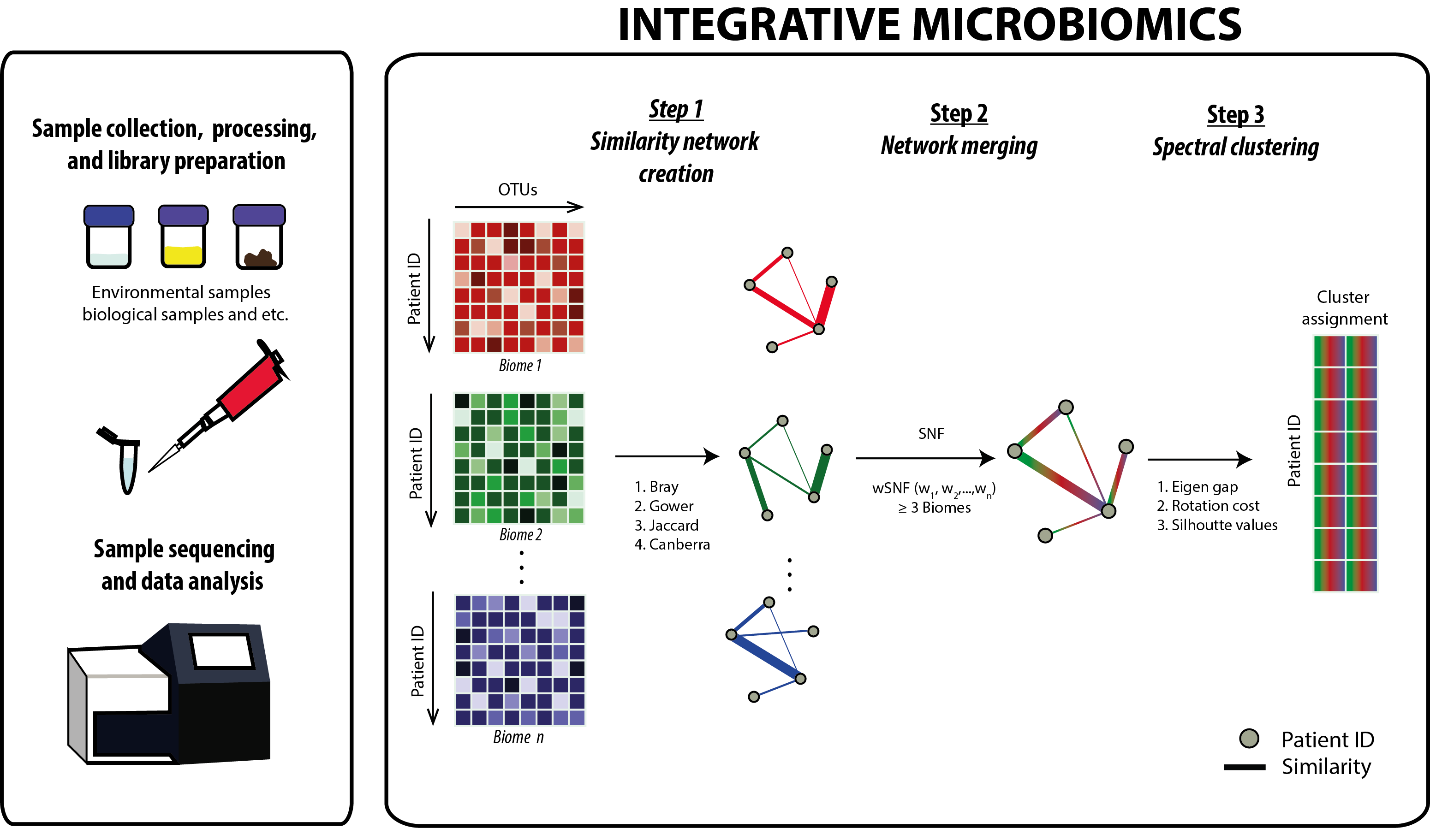
\includegraphics[width=\textwidth]{image/webtool_intro.png}
	\caption{A figure describing the workflow of integrative microbiomics. The input microbiome datasets, are converted into patient/sample similarity networks based on the user-specified similarity measures: 1) Bray-Curtis, 2) Gower, 3) Canberra and 4) Jaccard; before merging them using the user-specified algorithm: 1) SNF, 2) wSNF. Further, the tool then implements a spectral clustering algorithm to allow cluster analysis on the merged dataset.}
	\label{fig3}
\end{figure*}

Given the input microbiome datasets, the tool converts them into patient/sample similarity networks for each view based on the user-specified similarity measure before merging them using the user-specified algorithm. Further, the tool then implements a spectral clustering algorithm to allow cluster analysis on the merged dataset outputting the cluster assignments for each sample/patient. The optimum default number of clusters is computed using ensemble-based voting of three differing methodologies: Best Eigen Gap, Rotation cost and average silhouette method (Figure\ref{fig3}). For a given value of `k' (the number of clusters), we calculate a score/vote using the below rules

\begin{enumerate}
	\item If the average silhouette score > 0.7 $\rightarrow$ Score = Score + 3
	\item If 0.5 < average silhouette score < 0.7 $\rightarrow$ Score = Score + 2
	\item If 0.3 < average silhouette score < 0.5 $\rightarrow$ Score = Score + 1
	\item If k equals the first best value as derived from eigen gap method $\rightarrow$ Score = Score + 3
	\item If k equals the second-best value as derived from eigen gap method $\rightarrow$ Score = Score + 2
	\item If k equals the first best value as derived from rotation cost method $\rightarrow$ Score = Score + 3
	\item If k equals the second-best value as derived from rotation cost method $\rightarrow$ Score = Score + 2 
\end{enumerate} 
The value of k for which the Score is the highest is chosen as the default optimum number of clusters. In addition, the tool also outputs the integrated similarity matrix which can be used for downstream analysis such as for label propagation and survival analysis \cite{Wang2014}.

The tool presently provides four similarity measures 1) Bray-Curtis, 2) Gower, 3) Canberra and 4) Jaccard, appropriate for microbiome datasets which is used to construct patient/sample similarity network and two approaches 1) SNF, 2) wSNF to integrate these networks. For the implementation of wSNF the following formula in SNF
$$P^{(v)}=S^{(v)} \times \frac{\sum_{k=v} p^{k}}{(m-1)} \times (S^{(v)})^{T}, v=1,2,3, \ldots, m$$ was modified into $$P^{(v)}=S^{(v)} \times \frac{\sum_{k=v} \omega_{k} \times p^{(k)}}{\sum_{k \neq v} \omega_{k}} \times(S^{(v)})$$ $v=1,2,3, \ldots, m$
where $\omega_{k}$ is the weight of the $k^{ th}$ dataset, $m$ the total number of views, $P$ the status matrix and $S$ the kernel matrix as defined by Wang et.al \cite{Wang2014}.

This webtool allows the users to integrate multiple microbiome datasets obtained from different sites in a patient/biological entity or from various methods (targeted sequencing, metagenomics and qPCR) from the same site. For example, the lung microbiome (bacteria) with the gut microbiome (bacteria) or the lung microbiome (bacteria) with lung mycobiome. The tool assumes each input microbiome datasets represent a view of an underlying biological mechanism or a disease. Reliable estimation of each view is assumed when using SNF \cite{Jiang2019}. However, it may not always be practical to reliably estimate each view, although they play an equal role in the underlying biological process. This is due to the limitations and differing rates of development, in the present technologies and reference databases. In such cases, a weighted SNF approach is preferred, which still assumes the input datasets share an underlying biological mechanism but accounts for the inconsistency of the microbiome data based on the user-specified weights. The default weights are assigned based on the taxonomical richness (i.e. the number of microbes present) of the datasets. 

The interface of the webtool was developed using Rshiny and is available through Shiny Server (Open Source) in confluence with nginx-1.19.1. The tool is powered by custom scripts written in python2.7 and R; and containerized using Docker for ease of offline implementation. The developed webtool can be accessed at \url{https://integrative-microbiomics.ntu.edu.sg}.

\subsection{Longitudinal assessment of exacerbation}

A longitudinal cohort of n=17 patients were recruited from two hospitals in the east of Scotland (2016-2017) to study changes in the microbiome during exacerbation and following antibiotic treatment. DNA and RNA extraction were performed on sputum samples obtained from each patient and on a blank sterile PBS (Phosphate buffer solution). The extracted DNA was subjected to targeted amplicon sequencing of the 16S rRNA and ITS2 regions of the genome to derive the Microbiome and Mycobiome, by mapping them to green genes and UNITE databases, respectively. Blank samples contained read counts many orders of magnitude lower than test samples and hence unlikely to have any influence on the observed microbiome. RT-qPCR (real time quantitative polymerase chain reaction) was performed on the cDNA derived from the extracted RNA to quantify the viral burden of the 17 viruses investigated in each patient. $\alpha$ and $\beta$ diversity of the multi-biome was calculated from the concatenated microbiome and the integrated patient similarity matrix using the “vegan” package in R.

\subsection{Antibiotic action simulation}

To predict the impact of antibiotics on the interactome, $\beta$-lactam antibiotic action was simulated by a 75\% reduction in the relative abundance of the microbes targeted by this antibiotic in the baseline (pre-antibiotic) state including the following genera: \emph{Streptococcus, Staphylococcus, Haemophilus, Moraxella, Actinomyces, Arachnia, Bacteroides, Bifidobacterium, Eubacterium, Fusobacterium, Lactobacillus, Leptotrichia, Peptococcus, Peptostreptococcus, Propionibacterium, Selenomonas, Treponema and Veillonella}. In order to remove interactions resulting from random noise at the expense of sensitivity to weak signals and to allow comparison between the derived interactomes, the following abundance and prevalence filters were applied followed by co-occurrence analysis; retention of microbes present at greater than 1\% abundance in at least three subjects; in the pre OR post OR modelled antibiotic state.

\subsection{``Time to next exacerbation" prediction}

To predict “Time to next exacerbation”, Microbiome datasets were CLR (Centred log ratio) transformed before concatenation and microbes that are present in at least 4 patients at an abundance of 1\% were considered for further analysis. To derive pairwise microbial interactions for each patient, LIONESS \cite{Kuijjer2019}, a single patient network inference framework was implemented with General Boosted Linear model (GBLM) as the network inference algorithm. Correlation between the abundance of each microbes and interaction strength with ‘time to next exacerbation’ was assessed using Spearman’s rank correlation with statistical testing. Multivariate adaptive regression spline (MARS) \cite{Friedman1991}, a non-linear regression model was implemented with microbes or interaction strength as the predictor variable to predict ‘time to next exacerbation’ groups; defined as (Time to exacerbation: $<$12 weeks and $>$12weeks). The goodness of the fit of the model was evaluated by computing the R-squared (RSq) and the Generalized R-squared metric (GRsq). A feature importance plot based on Generalized Cross validation score (gcv) was also computed on the feature selected (microbes) by the model.  All the above analysis was implemented in R using the following packages 1)”Hmisc” 2) “earth” 3)”vegan” 4)”compositions” 5)”lionessR”.

\subsection{Validation of the interactome}

Experimental microbiological validation of Pseudomonas aeruginosa and Aspergillus fumigatus interaction was performed using one strain Aspergillus fumigatus (Af293) and three strains of Pseudomonas aeruginosa: (1) lab strain (PAO1) as control and (2,3) two clinical isolates of Pseudomonas aeruginosa derived from “low-risk” and “high-risk” patient clusters. The interaction was investigated using the disk inhibition method as described by Homa et al. \cite{Homa2019}.
An independent cohort of 166 patients was recruited from 4 sites (3 in Singapore and 1 in Dundee, Scotland) to validate the high-risk cluster and its interactome. DNA extraction was performed on the collected sputum samples of each patient. A shotgun metagenomic sequencing was performed at the NTU core sequencing facility on these samples according to the methods described by Gusareva et al. \cite{Gusareva2019}. Kaiju \cite{Menzel2016} with default parameters was implemented on the raw sequences after human read removal to estimate the taxonomic composition by referencing against NCBI BLAST nr+euk database. Estimation of the viruses that include prokaryotic phages and eukaryotic viruses was implemented using a custom pipeline that uses Demovir (\url{https://github.com/feargalr/Demovir}).
\section{Results}


\subsection {Math Cheat Sheet}
\begin{figure}
\begin{center}
    \begin{tikzpicture}
        \begin{axis}
            \addplot[color=red]{exp(x)};
        \end{axis}
    \end{tikzpicture}
    \caption{Plot of Exponential Function.}
    \label{fig:func1} % label must follow caption
\end{center}
\end{figure}



\hskip 5pt

\begin{figure}
\begin{center}
    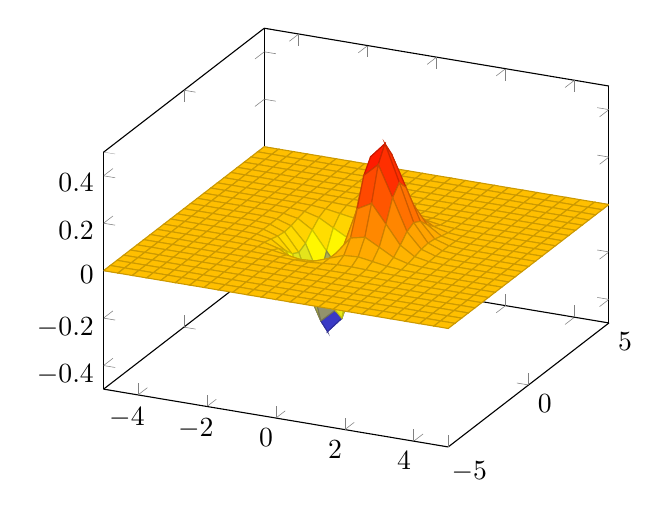
\begin{tikzpicture}
        \begin{axis}
            \addplot3[
                surf,
            ]
            {exp(-x^2-y^2)*x};
        \end{axis}
    \end{tikzpicture}
    \caption{Plot of 3-D Function.}
    \label{fig:func2}
\end{center}
\end{figure}

\begin{figure} [h!] 
    \centering
        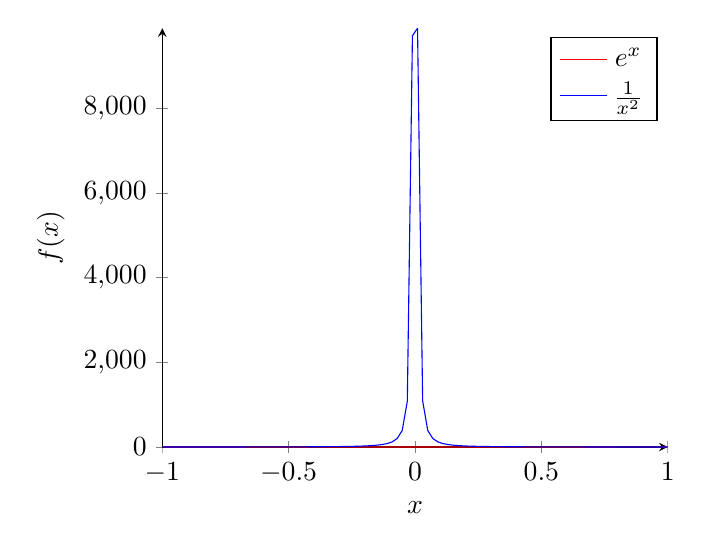
\begin{tikzpicture}
        \centering
        \begin{axis}[
            axis lines = left,
            xlabel = $x$,
            ylabel = {$f(x)$},
        ]
        %Below the red parabola is defined
        \addplot [
            domain=-1:1, 
            samples=100, 
            color=red,
        ]
        {e^x};
        \addlegendentry{$e^x$}
        %Here the blue parabola is defined
        \addplot [
            domain=-1:1, 
            samples=100, 
            color=blue,
            ]
            {1/x^2}; % note that the syntax here is different
        \addlegendentry{$\frac{1}{x^2}$}
        \end{axis}
        \end{tikzpicture}
        \caption{Two functions in one plot.}
        \label{fig:func3}
\end{figure}

\autoref{fig:func1}, \autoref{fig:func2}, and \autoref{fig:func3} are generated from function in \LaTeX. 


\subsection{Table Cheat Sheet}

\begin{table}[h]
    \centering
    \begin{tabular}{c|ccc}
        & Apple & Oranges & Strawberries \\
    \hline
    A & 1 & 2 & 3\\
    B & 1 & 2 & 3\\
    C & 1 & 2 & 3\\
    D & 1 & 2 & 3\\
    \end{tabular}
    \caption{Caption}
    \label{tab:my_label}
\end{table}

\section{Discussion}
In my master’s thesis, we presented to the best of our knowledge, the first ‘multi-biome’ analysis using ‘integrative microbiomics’ combining bacterial, viral, and fungal communities in individual patients. Using a modified weighted-SNF, we identified frequent exacerbators with high precision and classified microbes within an ‘interactome’ as ‘busy’, ‘influential’ and/or ‘critical’. Frequent exacerbators exhibited antagonistic interactomes. In my present PhD thesis, we extended this further by preforming a longitudinal assessment over an exacerbation. This reveal disrupted interactomes, undetectable by assessing microbial identity alone. By use of simulation followed by confirmatory validation, we demonstrate interactome’s clinical relevance for modelling microbiome re-configuration in response to antibiotic exposure. Validation of interactomes was achieved by metagenomics which identifies a cluster that exhibits, a similar high-risk of exacerbation phenotype as identified from the derivation cohort. Further, interactome analysis of the high-risk cluster derived using the metagenomic validation cohort validates 89.9\% of the interactions. We also, provide microbiological evidence in support of our interactome approach by demonstrating variable interaction between \emph{P. aeruginosa} and \emph{A. fumigatus} using cluster-specific clinical isolates. We then assessed the clinical applicability of the interactome by modelling time to next exacerbation using interactions and individual taxa as features. Interestingly, we find a major increase in the accuracy of prediction when using interactions, in contrast to individual taxa. Taken together, our findings reveal a novel aspect of the functional microbiome with potential implications for the use of antibiotics in clinical practice.

It is well recognised in bronchiectasis, that patients improve despite receiving antibiotics not necessarily targeting their dominant pathogen. However, the conventional model where targeting bacteria with antibiotics reduces bacterial load, accompanying inflammation and therefore, exacerbation risk, which, in turn, alleviates symptoms and improves clinical outcomes; fails to explain this. If the interactome framework were true, then this could offer explanations of unexplained clinical observations of antibiotic use and help treat exacerbations. Results from this study show that interactions are more predictive than individual taxa of time to next exacerbation and better explain exacerbation, in support of the hypothesis. The airway microbiome (and its accompanying interactome) is likely a critical predictor of antibiotic treatment response and provides a theoretical basis for understanding several phenomena associated with antibiotics that remain unexplained clinically including antimicrobial responses in apparently resistant organisms. Manipulating microbiomes by means other than antibiotics are being explored and the effect of probiotics on the interactome should be considered.

The value of data integration using SNF for multidimensional datasets (such as multi-omics) in airways disease such as COPD has been demonstrated; however, these methods have not been previously applied to microbiome integration \cite{Li2018}. Conventional SNF is not optimized for biological systems such as multi-kingdom microbiomes where dynamism and potential dominance of one kingdom over the others needs to be considered. Employing a weighted SNF approach based on richness, we demonstrate improved patient stratification in bronchiectasis by identifying high frequency exacerbators with accuracy exceeding that of using a single microbial group. Hence to motivate and enable; researchers and clinicians to opt for an integrative strategy when analysing multi biome datasets, we developed a web tool “Integrative Microbiomics” (\url{https://integrative-microbiomics.ntu.edu.sg}) capable of implementing both SNF and weighted SNF to integrate microbiome datasets. This webtool also aims to motivate users to obtain multi biome datasets, as integrating datasets would better represent/ bring clarity to the underlying biological process. 

Limitations of this work include the cross-section design of the CAMEB cohort, a static dataset which we largely use to predict dynamic interaction \cite{Aogain2019,Mac1800766}. However, this is partially overcome by the inclusion of a longitudinal case series to our analysis to better assess temporal dynamics in association to exacerbation and antibiotic treatment. Next, although 16S methodologies are well established, there are inherent limitations, including under-representation of mycobacteria, an important group of organisms in bronchiectasis \cite{Sulaiman2018}. Additionally, fungal ITS sequencing approaches are challenged by under-developed reference databases \cite{Ali2019}. Our virome analysis, while broad, comprehensive, and informed by established literature, targets a known virus panel and therefore is subject to bias. Nonetheless, this is partially addressed by our metagenomic dataset, which comprehensively assess the virome. While metagenomics potentially represents a less biased alternative approach, it underestimates fungal presence given the significantly higher airway bacterial burden hence obscuring the influence that fungi have on the interactome. We further acknowledge that sputum is an imperfect matrix, and, make no inference about lower airway ecology, noting only the clinical associations between sputum as a surrogate, readily obtainable, non-invasive upper airway sample. Finally, while observational data suggests potential causal association, other factors may drive observed effects. Observed interactions may represent epiphenomena of a selectively operating immune system, for example and our work did not include any assessment of host responses.
\section{Future works}
Lorem ipsum dolor sit amet, consectetuer adipiscing elit. Aenean commodo ligula eget dolor. Aenean massa. Cum sociis natoque penatibus et magnis dis parturient montes, nascetur ridiculus mus. Donec quam felis, ultricies nec, pellentesque eu, pretium quis, sem. Nulla consequat massa quis enim. Donec pede justo, fringilla vel, aliquet nec, vulputate eget, arcu. In enim justo, rhoncus ut, imperdiet a, venenatis vitae, justo. Nullam dictum felis eu pede mollis pretium. Integer tincidunt. Cras dapibus. Vivamus elementum semper nisi. Aenean vulputate eleifend tellus. Aenean leo ligula, porttitor eu, consequat vitae, eleifend ac, enim. Aliquam lorem ante, dapibus in, viverra quis, feugiat a, tellus. Phasellus viverra nulla ut metus varius laoreet. Quisque rutrum. Aenean imperdiet. Etiam ultricies nisi vel augue. Curabitur ullamcorper ultricies nisi. Nam eget dui. Etiam rhoncus. Maecenas tempus, tellus eget condimentum rhoncus, sem quam semper libero, sit amet adipiscing sem neque sed ipsum. Nam quam nunc, blandit vel, luctus pulvinar, hendrerit id, lorem. Maecenas nec odio et ante tincidunt tempus. Donec vitae sapien ut libero venenatis faucibus. Nullam quis ante. Etiam sit amet orci eget eros faucibus tincidunt. Duis leo. Sed fringilla mauris sit amet nibh. Donec sodales sagittis magna. Sed consequat, leo eget bibendum sodales, augue velit cursus nunc, quis gravida magna mi a libero. Fusce vulputate eleifend sapien. Vestibulum purus quam, scelerisque ut, mollis sed, nonummy id, metus. Nullam accumsan lorem in dui. Cras ultricies mi eu turpis hendrerit fringilla. Vestibulum ante ipsum primis in faucibus orci luctus et ultrices posuere cubilia Curae; In ac dui quis mi consectetuer lacinia. Nam pretium turpis et arcu. Duis arcu tortor, suscipit eget, imperdiet nec, imperdiet iaculis, ipsum. Sed aliquam ultrices mauris. Integer ante arcu, accumsan a, consectetuer eget, posuere ut, mauris. Praesent adipiscing. Phasellus ullamcorper ipsum rutrum nunc. Nunc nonummy metus. Vestibulum volutpat pretium libero. Cras id dui. Aenean ut \cite{kingma2014adam}
\newpage
\chapter{Microbial dysregulation of the `lung-gut' axis in high-risk bronchiectasis}
\section{Introduction}

The term microbiome is used to refer to the collection of genes within a community of microbes (including bacteria, fungi, virus, protists and bacteriophages). In the last few years, microbiome research has helped us gained new insights into how microbes shape our human biology and have brought paradigm-shifting implications for translational research and clinical care. The human microbiota is crucial for our body to maintain its homeostasis. Disruption of this can lead to diseases such as obesity, inflammatory bowel disease, malnutrition, Parkinson's, Autism, Asthma, dental caries, bacterial vaginosis, and depression \cite{Knight2017}.  Currently, microbiome researchers use culture-independent techniques that involve DNA sequencing to derive the microbiome. Broadly, the community taxonomy/microbiome can be identified using two approaches (see Figure\ref{fig1}) 1) Targeted and 2) Metagenomic. Targeted sequencing approach uses the PCR amplified, target gene markers (16S rRNA in case of bacteria or ITS in case of Fungi) derived from the samples to reference it against gene-marker databases (Silva, Green Genes, etc.). In contrast, the metagenomic sequencing approach directly sequence the whole community DNA and compares it to reference genomes \cite{Morgan2012}.

\begin{figure}[ht]
	\centering
	\includegraphics[width=0.5\textwidth]{./image/introduction.png}
	\caption{A figure illustrating the different sequencing approaches used to derive the human microbiome, consisting of interacting bacteria, fungi and viruses. Adapted from: \cite{Morgan2012}}
	\label{fig1}
\end{figure}

Present microbiome studies focus on a single profile of the human microbiome in isolation, even though bacteria, fungi and viruses coexist and interact in the body as a community. Thus, it is essential to look at these biological components together in an integrated fashion to understand more holistically the true underlying in vivo state. However, one of the primary reasons for the lack of multi-biomic research is the lack of methods to merge microbiome datasets and integrative analysis. Consequently, I tried addressing some of these challenges in my master's thesis, using microbiome datasets derived from bronchiectasis patients as an example. Bronchiectasis, is a chronic inflammatory respiratory disease associated with progressive, irreversible dilatation of the airway. It is crucial to study bronchiectasis because in most cases it is known to be idiopathic(unknown cause) \cite{pmid29478908} and it is a significant contributor to lung diseases globally with a substantial four-fold higher predominance in Asian populations \cite{Seitz2012}. 

\begin{figure*}[!h]
	\centering
	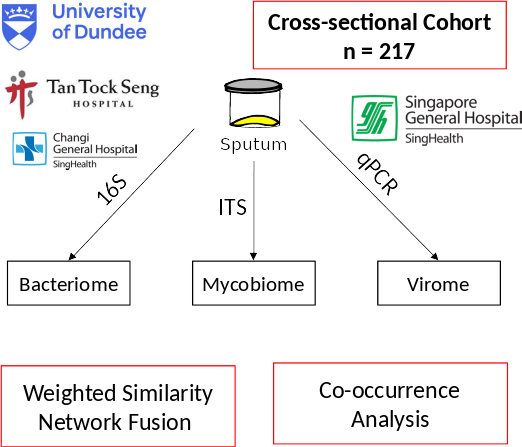
\includegraphics[width=0.50\textwidth]{./image/methods_masters.png}%
	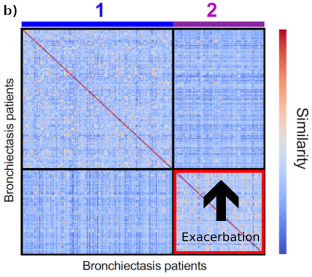
\includegraphics[width=0.50\textwidth]{./image/Res2.png}\\
	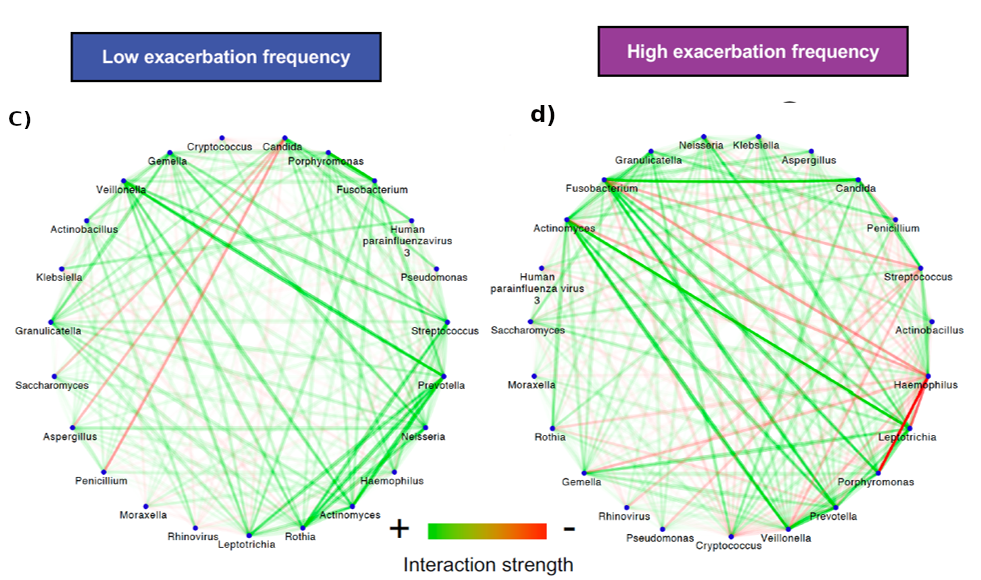
\includegraphics[width=\textwidth]{./image/Res3.png}
	\caption{(a) A schematic representing, overview of analysis performed on the CAMEB cohort (n=217). Methodologies: Weighted SNF and Co-occurrence analysis were used for microbiome integration and intreactome construction. (b) A patient similarity matrix with each cell representing the integrated similarity between patients. Two clusters of low (black) and high (red) risk patients identified by wSNF are highlighted by boxes. Visualization of the interactome of low (c) and high (d) risk clusters. Interactions between microbes are	classified as negative if the sign of the edge weights between them is negative (coloured red) with positive interactions indicated by green colouration. The strength of the interaction is indicated by the colour depth}
	\label{fig2}
\end{figure*}

Previously in my master's thesis, I developed weighted similarity network fusion (wSNF) to allow weightage of input datasets during integration, otherwise unaccounted by conventional SNF \cite{Wang2014}. Ensemble-based co-occurrence analysis strategy developed by Faust et al. \cite{Faust2012} was extended to allow weightage of individual methods in the ensemble along with other modification to better infer microbial association networks. Microbiome and Mycobiome derived using targeted amplicon sequencing of the 16S and ITS regions from the sputum samples of the CAMEB cohort \cite{Mac1800766}; virome from qPCR on an extensive panel of 17 respiratory viruses, were used as the example dataset to integrate the microbiomes (Figure\ref{fig2}a). Multi-biome (Microbiome, Mycobiome and Virome) integration by wSNF identifies a high-risk exacerbation cluster with increased precision (Figure\ref{fig2}b). Co-occurrence network analysis of this high-risk cluster revealed an elevated antagonistic interactome with reduced alpha-diversity (Figure\ref{fig2}c) \cite{Narayana2019}.

Having developed the wSNF and shown its increased precision to identify exacerbators (clinical outcomes); here in my PhD thesis, I attempt to extend my results further. I aim to develop a web tool to enable users to integrate their microbiome datasets and to illustrate its advantages using publicly available microbiome datasets. The tool would motivate clinicians and microbiome researchers to explore multi-biome strategies for their problem and aid them in integrating their datasets. Secondly, I aim to study exacerbation events, antimicrobial perturbations and ``Time to next exacerbation" using the developed ``Interactome" framework. Thirdly, I aim to validate the ``high-risk" exacerbation cluster of Bronchiectasis patients and its ``interactome" as derived in my previous work \cite{Narayana2019} using an alternate sequencing approach: metagenomics. Further, we also pick an interaction from the interactome of the high and low-risk clusters and validate it experimentally. 
\section{Methods}


\section{Results}

\subsection{Significant overlap of fungal communities of lung and gut contrary to bacteria}

Intersection analysis of bacterial and fungal communities between sputum and stool samples reveals increased overlap of fungal communities between the lung and gut, contrary to bacteria. Three bacterial genera including \emph{Lactobacillus, Prevotella} and \emph{Streptococcus} compared to six fungal genera including \emph{Candida, Cryptococcus, Curvularia, Debaryomyces, Lodderomyces} and \emph{Saccharomyces} were present in both sputum and stool samples. Interestingly, upon assessment of diversity between the sputum and stool samples, a similar pattern is observed. Overall, mycobiome exhibits a decreased diversity compared to microbiome. Further, an increased diversity of bacteria is found in the gut compared to the lung whereas the fungal diversity doesn't change. 

\begin{figure}[h]
	\centering
	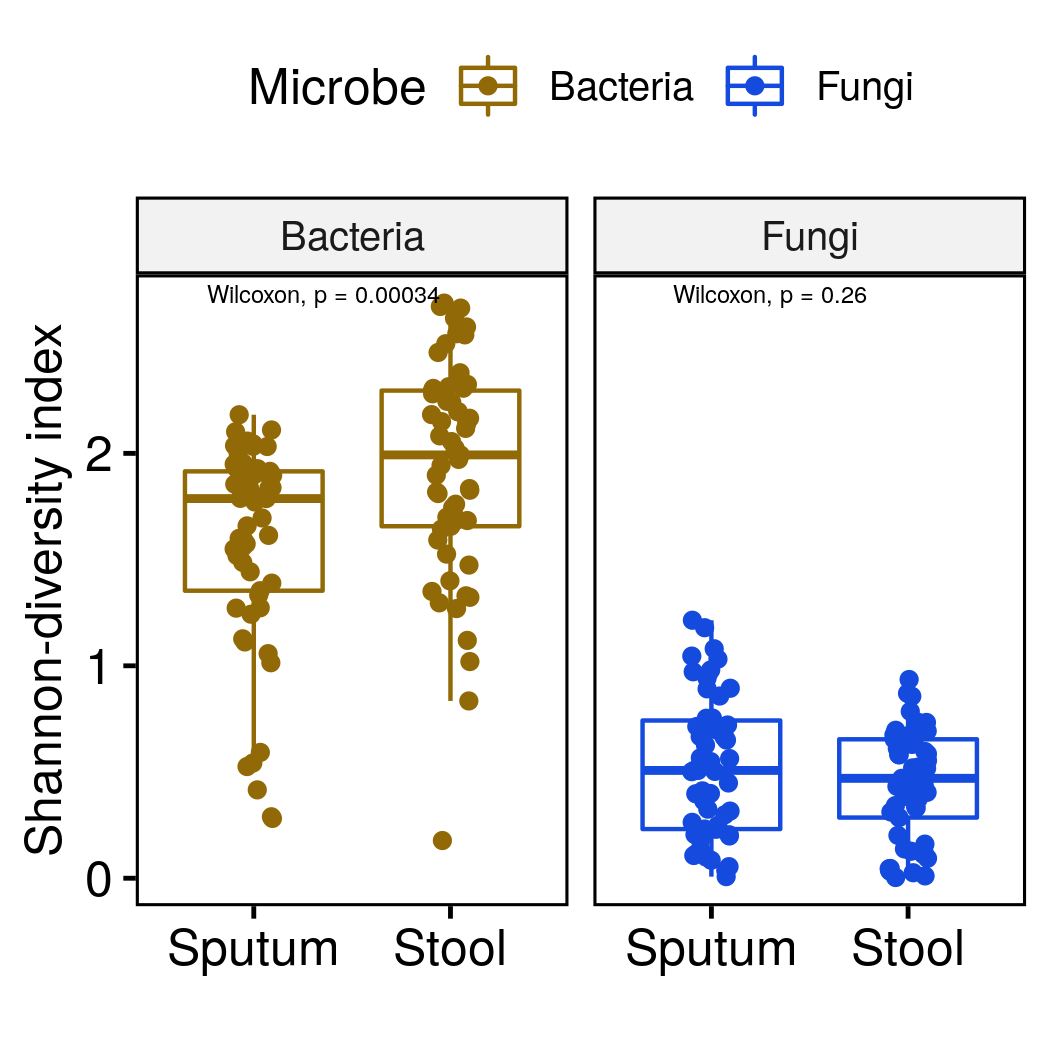
\includegraphics[width=0.5\textwidth]{image/diversity.png}
	\caption{A boxplot illustrating the difference in Shannon-diversity index of the Microbiome (Ochre) and Mycobiome (Blue) between the sputum (Lung) and stool (Gut) samples. Statistical significance of these differences were calculated using `wilcoxon test' and are indicated above as p-values.}
	\label{res2_fig1}
\end{figure}

\subsection{Co-occurrence analysis reveals lung – gut microbial (bacteria and fungi) interactions suggestive of a potential lung-gut axis.}


MOFA2 analysis reveals factors, highly contributed by the Gut bacteria and associated with exacerbations. 

Integrating microbiomes (bacteria and fungi) from lung and the gut, following clustering identifies patients with increased risk of exacerbation, Reiff score and FACED with no difference in lung function. 

High-risk patients exhibit significantly increased \emph{Candia} in Gut, \emph{Fusobacterium} in Lung, increased lung-gut microbial interaction (35\%>29\%) and movement of Streptococcus between lung and gut, illustrating a dysregulated lung-gut axis.
\newpage
\section{Discussion}
In my master’s thesis, we presented to the best of our knowledge, the first ‘multi-biome’ analysis using ‘integrative microbiomics’ combining bacterial, viral, and fungal communities in individual patients. Using a modified weighted-SNF, we identified frequent exacerbators with high precision and classified microbes within an ‘interactome’ as ‘busy’, ‘influential’ and/or ‘critical’. Frequent exacerbators exhibited antagonistic interactomes. In my present PhD thesis, we extended this further by preforming a longitudinal assessment over an exacerbation. This reveal disrupted interactomes, undetectable by assessing microbial identity alone. By use of simulation followed by confirmatory validation, we demonstrate interactome’s clinical relevance for modelling microbiome re-configuration in response to antibiotic exposure. Validation of interactomes was achieved by metagenomics which identifies a cluster that exhibits, a similar high-risk of exacerbation phenotype as identified from the derivation cohort. Further, interactome analysis of the high-risk cluster derived using the metagenomic validation cohort validates 89.9\% of the interactions. We also, provide microbiological evidence in support of our interactome approach by demonstrating variable interaction between \emph{P. aeruginosa} and \emph{A. fumigatus} using cluster-specific clinical isolates. We then assessed the clinical applicability of the interactome by modelling time to next exacerbation using interactions and individual taxa as features. Interestingly, we find a major increase in the accuracy of prediction when using interactions, in contrast to individual taxa. Taken together, our findings reveal a novel aspect of the functional microbiome with potential implications for the use of antibiotics in clinical practice.

It is well recognised in bronchiectasis, that patients improve despite receiving antibiotics not necessarily targeting their dominant pathogen. However, the conventional model where targeting bacteria with antibiotics reduces bacterial load, accompanying inflammation and therefore, exacerbation risk, which, in turn, alleviates symptoms and improves clinical outcomes; fails to explain this. If the interactome framework were true, then this could offer explanations of unexplained clinical observations of antibiotic use and help treat exacerbations. Results from this study show that interactions are more predictive than individual taxa of time to next exacerbation and better explain exacerbation, in support of the hypothesis. The airway microbiome (and its accompanying interactome) is likely a critical predictor of antibiotic treatment response and provides a theoretical basis for understanding several phenomena associated with antibiotics that remain unexplained clinically including antimicrobial responses in apparently resistant organisms. Manipulating microbiomes by means other than antibiotics are being explored and the effect of probiotics on the interactome should be considered.

The value of data integration using SNF for multidimensional datasets (such as multi-omics) in airways disease such as COPD has been demonstrated; however, these methods have not been previously applied to microbiome integration \cite{Li2018}. Conventional SNF is not optimized for biological systems such as multi-kingdom microbiomes where dynamism and potential dominance of one kingdom over the others needs to be considered. Employing a weighted SNF approach based on richness, we demonstrate improved patient stratification in bronchiectasis by identifying high frequency exacerbators with accuracy exceeding that of using a single microbial group. Hence to motivate and enable; researchers and clinicians to opt for an integrative strategy when analysing multi biome datasets, we developed a web tool “Integrative Microbiomics” (\url{https://integrative-microbiomics.ntu.edu.sg}) capable of implementing both SNF and weighted SNF to integrate microbiome datasets. This webtool also aims to motivate users to obtain multi biome datasets, as integrating datasets would better represent/ bring clarity to the underlying biological process. 

Limitations of this work include the cross-section design of the CAMEB cohort, a static dataset which we largely use to predict dynamic interaction \cite{Aogain2019,Mac1800766}. However, this is partially overcome by the inclusion of a longitudinal case series to our analysis to better assess temporal dynamics in association to exacerbation and antibiotic treatment. Next, although 16S methodologies are well established, there are inherent limitations, including under-representation of mycobacteria, an important group of organisms in bronchiectasis \cite{Sulaiman2018}. Additionally, fungal ITS sequencing approaches are challenged by under-developed reference databases \cite{Ali2019}. Our virome analysis, while broad, comprehensive, and informed by established literature, targets a known virus panel and therefore is subject to bias. Nonetheless, this is partially addressed by our metagenomic dataset, which comprehensively assess the virome. While metagenomics potentially represents a less biased alternative approach, it underestimates fungal presence given the significantly higher airway bacterial burden hence obscuring the influence that fungi have on the interactome. We further acknowledge that sputum is an imperfect matrix, and, make no inference about lower airway ecology, noting only the clinical associations between sputum as a surrogate, readily obtainable, non-invasive upper airway sample. Finally, while observational data suggests potential causal association, other factors may drive observed effects. Observed interactions may represent epiphenomena of a selectively operating immune system, for example and our work did not include any assessment of host responses.
\newpage
\chapter*{Future works}
\addcontentsline{toc}{chapter}{Future works}

The developed and validated interactome framework is based on “Graph theory”, a mathematical theory that study graphs as basic structures to model pairwise relation of nodes as points. Besides, mathematics also provides a generalisation of Graphs through “Simplicial complexes” from the field of Algebraic topology. A simplicial complex is a mathematical structure that models pairwise relation of simplices (generalisation of nodes), which captures complex relationships as points, lines, triangles and their n-dimensional counterparts. Given that interactions of nodes (microbes) are beneficial than isolated microbes in studying clinical outcomes such as exacerbations and antibiotic action; as my next step, I would like to test the hypothesise that the simplicial complex framework is more beneficial than the interactome framework, to study important clinical outcomes. We have shown that the post-exacerbation (post-antibiotic) interactome is predictive of time to next exacerbation with a GRsq (Generalised R Squared) of 55\%, if the proposed hypothesis were true, this could lead to increased accuracy of prediction. Secondly, I also plan on implementing powerful prediction models that are based on machine learning to further increase the accuracy to predict clinical outcomes, advancing the field of precision medicine. Further, I am planning to submit an ERJMethods paper detailing methods such as Similarity Network Fusion (SNF) to integrate datasets.

\pagenumbering{arabic}

\newpage
\bibliographystyle{acm}
\bibliography{reference}

\end{document}